\documentclass[11pt]{article}

\usepackage{amsmath}
\usepackage{amssymb}
\usepackage{graphicx}

\newcommand{\code}[1]{\texttt{#1}}

\begin{document}

\author{Gu, Qiao}
\title{16-720B Homework 1 Write-up}
\maketitle

\medskip

\subsection*{Q1.1.1}

\newpage

\subsection*{Q1.1.2}

Please see the Figure~\ref{fig:q1.1.2} for the filter responses

\begin{figure}[h!]
    \centering
    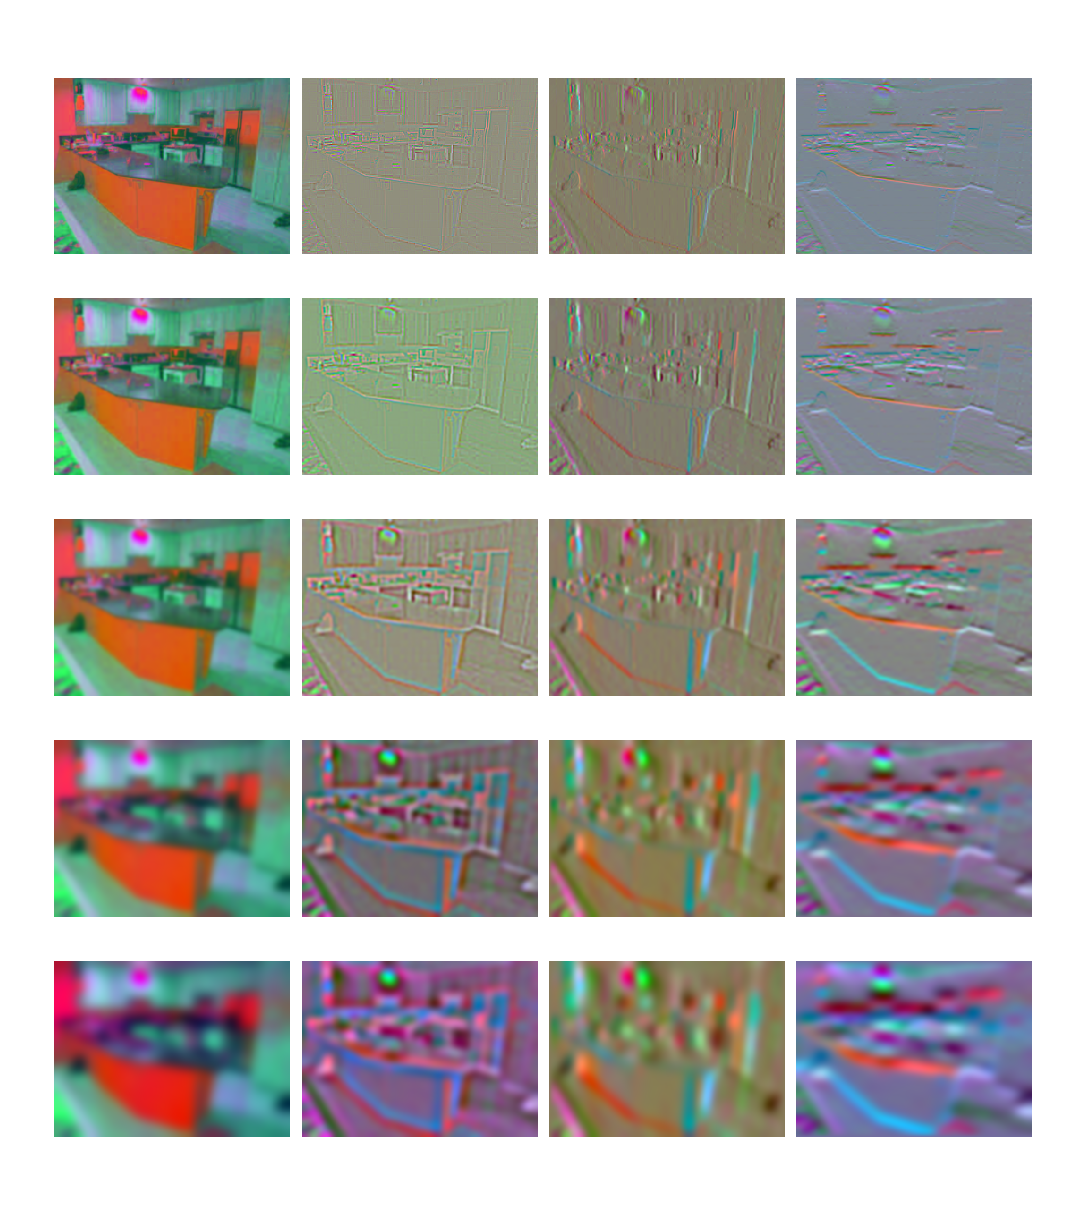
\includegraphics[width=\linewidth]{../results/q1_1_2_responses.png}
    \caption{Filter responses on the image \code{aquarium/sun aztvjgubyrgvirup.jpg}. }
    \label{fig:q1.1.2}
\end{figure}

\newpage

\subsection*{Q1.3}

\newpage

\subsection*{Q2.5}

The overall accuracy is $0.64375$, and the confusion matrix is as follows:

\begin{verbatim}
  [[14.  0.  0.  0.  0.  0.  0.  0.]
   [ 0. 14.  0.  1.  0.  1.  2.  0.]
   [ 0.  0. 15.  4.  3.  0.  0.  3.]
   [ 1.  2.  1. 17.  0.  0.  1.  4.]
   [ 1.  1.  0.  0. 10.  1.  0.  0.]
   [ 0.  2.  0.  1.  8. 12.  1.  0.]
   [ 0.  5.  0.  0.  2.  3. 11.  0.]
   [ 0.  2.  3.  2.  1.  1.  0. 10.]]
\end{verbatim}

\newpage

\subsection*{Q2.6}

\newpage



\end{document}
